% Asset ID: AS2MeasuresLocationSpreadTikZ-002
% Purpose: Show interpolation as a frequency fraction mapped to a class-interval fraction.
\documentclass[tikz,border=8pt]{standalone}
\usepackage{amsmath}
\usetikzlibrary{arrows.meta, positioning, calc}
\begin{document}
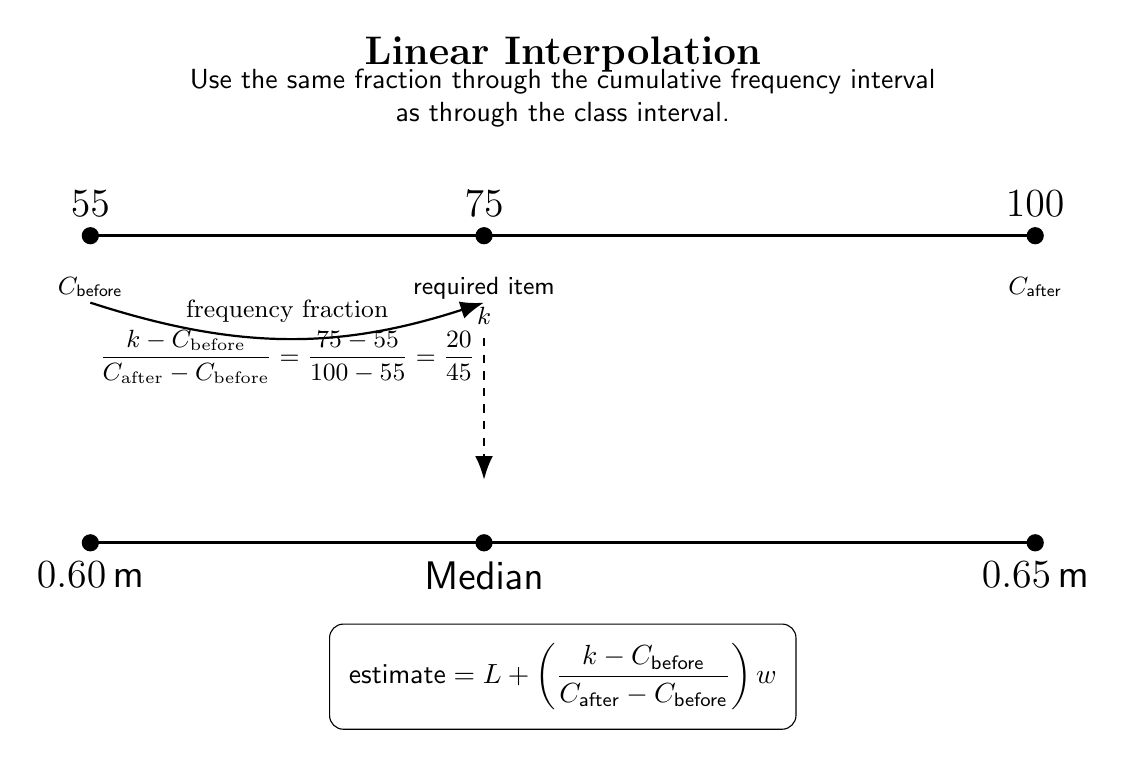
\begin{tikzpicture}[font=\sffamily, dot/.style={circle, fill=black, inner sep=2.2pt}, lab/.style={align=center, font=\small\sffamily}]
\node[font=\Large\bfseries] at (0,4.6) {Linear Interpolation};
\node[align=center] at (0,4.05) {Use the same fraction through the cumulative frequency interval\\as through the class interval.};
\draw[line width=1.2pt] (-6,2.3) -- (6,2.3);
\node[dot, label=above:{\Large $55$}] at (-6,2.3) {};
\node[dot, label=above:{\Large $75$}] at (-1.0,2.3) {};
\node[dot, label=above:{\Large $100$}] at (6,2.3) {};
\node[lab, below=4mm] at (-6,2.3) {$C_{\text{before}}$};
\node[lab, below=4mm] at (-1.0,2.3) {required item\\$k$};
\node[lab, below=4mm] at (6,2.3) {$C_{\text{after}}$};
\draw[-{Latex[length=3mm]}, thick] (-6,1.45) to[bend right=18] (-1.0,1.45);
\node[align=center, font=\small] at (-3.5,0.95) {frequency fraction\\[2pt]$\displaystyle \frac{k-C_{\text{before}}}{C_{\text{after}}-C_{\text{before}}}=\frac{75-55}{100-55}=\frac{20}{45}$};
\draw[-{Latex[length=3mm]}, thick, dashed] (-1.0,1.0) -- (-1.0,-0.8);
\draw[line width=1.2pt] (-6,-1.6) -- (6,-1.6);
\node[dot, label=below:{\Large $0.60\,\text{m}$}] at (-6,-1.6) {};
\node[dot, label=below:{\Large Median}] at (-1.0,-1.6) {};
\node[dot, label=below:{\Large $0.65\,\text{m}$}] at (6,-1.6) {};
\node[draw, rounded corners=5pt, align=center, inner sep=7pt] at (0,-3.3) {$\displaystyle \text{estimate}=L+\left(\frac{k-C_{\text{before}}}{C_{\text{after}}-C_{\text{before}}}\right)w$};
\end{tikzpicture}
\end{document}
